%*************************************************
\section{Approximate query processing}
\label{sec:ApproximateQueryProcessing}
%*************************************************

On-Line Analytical Processing (OLAP) systems process large volumes of data to produce information regarding the operations of enterprises. Such applications extract data from  massive datasets, but the response time for searching the entire database restricts the usefulness of data analytics. A useful alternative approach is offered  by the Approximate Query Processing (AQP) \cite{Agarwal:2014:KYW:2588555.2593667}.

AQP is a sampling technique for providing approximate responses to aggregated queries. An aggregate query is a query that calls aggregate functions to return a computed summary with significant meaning from the value of attributes of a group of documents. Common aggregate functions are: {\it Average, Max, Min}, and {\it Count}. An AQP system supplies confidence intervals indicating the percentage of uncertainty of the approximate answers along with the responses.  

AQP can be extremely useful for minimizing the information leakage of very large databases.  One of the methods to prevent information leakage is replication of database documents with sensitive information, using altered data for the sensitive  fields.  The larger the replication factor, the more difficult is for an attacker to identify the sensitive information, but  the larger is the storage for the expanded database. For example, a $100$ TB database  becomes $1$ PB database for a replication factor of ten.

The indiscriminate replication of all database documents, not only increases the storage space dramatically, but also increases the response time for aggregate queries by a factor which is at least equal to the replication factor. Such an indiscriminate replication is not warranted as the documents have different levels of sensitivity. The alternative solution proposed in this paper requires a \emph{sensitivity analysis} of the database documents. This analysis allows us to selectively apply disinformation to the database documents.

Sensitivity analysis has two stages, (i) establish a number of sensitivity levels and (ii) determine the number of database documents at each sensitivity level. The second stage of the sensitivity analysis requires an examination of all database documents which is a slow process, and infeasible for real-time OLAP applications. Instead of a prolonged aggregation, we proposed using AQP to facilitate fast sensitivity analysis over samples with inaccuracy within acceptable ranges. Observations in the samples are randomly selected from the original database and queries are directed against these small samples in parallel manner.\\

For a given aggregate query $\theta$, $S$ is a set of $n$ sensitivity classes of documents in the collection, $S=\{s_1 \dots s_n\}$, and the exact count of each sensitivity class $s_i$ is presented by $c_i$, such that $C=\{c_1 \dots c_n\}$. Consider the response $R$ for the approximate query $\hat{\theta}$ that constitutes a set of $m$ sensitivity classes denoted as $S^\prime=\{s_1^\prime \dots s_m^\prime\}$ with the corresponding approximated count values of $C^\prime=\{c_1^\prime \dots c_m^\prime\}$. In a uniform random sampling from $n$ classes of documents, it is possible to have only $m$ classes in approximated response ($n\ge m$); thus, $n-m$ classes are not appeared in the response \cite{babcock2003dynamic}. The probability of having missed classes in $R$ is defined as : 

\begin{equation} 
\label{equ:ProbabilityMissedClass}
\begin{aligned}
P(\hat{\theta}, R)= \frac{n-m}{m}
\end{aligned}
\end{equation}
The average error on $R$ of $\hat{\theta}$ is presented as :
\begin{equation} 
\label{equ:RelativeError}
\begin{aligned}
Error(\hat{\theta}, R)=\frac{1}{n}\bigg( (n-m)+ \sum_{j=1}^{m} \frac{\mid c_j-c_j^\prime \mid}{c_j} \bigg)  
\end{aligned}
\end{equation}


Random sampling for approximate measurement is a known solution that dramatically cuts the analysis time, especially if the sample is small enough to fit in the main memory of the system. However, approximate measurements based on random sampling only approximates real database measurements. The Sampling-based Approximate Query Processing (S-AQP) with guaranteed accuracy provides bounds on the error caused by sampling \cite{Agarwal:2014:KYW:2588555.2593667}. Periodically assessing the information leakage from large datasets tolerates a certain degree of inaccuracy. The AQP is used for sensitivity analysis and fast leakage parameter extraction with minimum inaccuracy, while reducing the query response time.

%**************************************************************
\subsection{Error bounds}
\label{ErrorBoundsSubsection}
%*********************************************************

A key element of any AQP system is to provide error bounds for the approximative results,    allowing the user to decide whether the results are acceptable. \emph{Confidence Intervals} (CI) a.k.a error bar which is a range of values that are centered at a known sample mean are used to calculate error bounds. We use a close-form Central Limit Theorem(CLT) and two other large deviation inequalities, namely Markov and Chebyshev inequalities to get the tightest bounds. We use Markov inequality to obtain a better bound than the trivial one of $1.0$.  Additional information on the variance improves the bounds given by Chebyshev inequality. As the number of elements in the sample $n$ goes to infinity, the distribution converges into the standard normal random distribution $N(0,1)$. The close-form CLT approach is shown in Equation \ref{equ:CLT}. 

\begin{equation} 
\label{equ:CLT}
\begin{aligned}
\Big(\frac{\sum_{i=1}^n X_i - \mathbb{E}\big[\sum_{i=1}^n X_i\big]}{\sqrt{\mathrm{Var}(\sum_{i=1}^n X_i)}}\Big)\xRightarrow[\text{}]{n\to\infty } N(0,1)
\end{aligned}
\end{equation}
Where $\mathbb{E}$ is expected value (or mean) of a discrete random variable $X_i$.  

The tightness of the bounds resulted from the three aforementioned approaches are illustrated in Figure \ref{fig:inequalites}. Comparing these three approaches, it is found that Markov's inequality provides larger deviation bounds than ChebyShev's inequality. Close-form CLT provides the tightest bound among these three approaches \cite{huber1967behavior}.

\begin{figure}[H]
\centering
\resizebox{0.6\textwidth}{!}{\begin{tikzpicture}[scale=1.1,thick]
\usetikzlibrary{calc}
\coordinate (A) at (-5,2.5);
\node at (A) [above = 2mm of A] {\Large $0$};

\coordinate (B) at (5,2.5);
\node at (B) [above = 2mm of B] {\Large $1$};

\draw[decorate,decoration={brace,raise=35pt,amplitude=5pt}] 
  (A) -- node[fill=white, inner sep=1pt,above left=45pt and -50pt]{Tightness of bounds} (B);


\draw [line width=0.35mm,black](A)--(B)[right];
\draw[densely dotted] (3,2.8) -- (3,2.2) node [below] {Markov inequality}; 
\draw[densely dotted] (3.01,2.8) -- (3.01,2.2);

\draw[densely dotted] (0,2.8) -- (0,1.5) node [below] {Chebyshev's inequality};
\draw[densely dotted] (0.01,2.8) -- (0.01,1.5);

\draw[densely dotted] (-4,2.8) -- (-4,0.8) node [below] {CLT close-form};
\draw[densely dotted] (-4.01,2.8) -- (-4.01,0.8);

\fill [purple] (A) circle (4pt);
\fill [purple] (B) circle (4pt);
\end{tikzpicture}
}
\caption{General comparison between tightness of bounds resulting from Markov, ChebyShev's inequalities and close-form CLT.}
\label{fig:inequalites}
\end{figure}


%*************************************************
\subsection{Sampling methods}
\label{SamplingMethodsSubsection}
%*************************************************

In the {\it sampling phase}, observations can be selected by sampling with or without replacement. In the sampling without replacement (disjoint samples), any two samples are independent thus, their covariance is zero. In sampling with replacement, the two sample values are dependent such that the observations in the first sample affects what we can get for the second one and the covariance of the two is not zero. The sampling without replacement complicates the sampling process, but it leads to a slightly more accurate estimation. The resampling process can be extended to multiple levels to satisfy any user defined constraints  such as latency or accuracy. Sampling allows AQP to meet low latency and error percentage requirements. If a user rejects the approximative results of AQP due to deviation from the expected criteria, the next step is to switch to the larger samples as a new working set, so that eventually the expected results are obtained. 


A bootstrap like resampling method is required to create a multi-layer sample set to meet different expectations. Assume $\theta$ is the query which is posed to process on the very large database $D$. With AQP the new query $\hat{\theta}$ will be composed to approximate the answer of $\theta$ using proper sample set. To rewrite an aggregate query $\theta$ to $\hat{\theta}$, one of the critical parameter is the scaling factor, denoted as $\delta=\frac{\mid D\mid}{\mid sample \mid}$ which is the ratio of the cardinality of the original database to cardinality of the sample. Figure \ref{samplingFigure} presents our resampling method we use for the experiments \cite{Agarwal:2014:KYW:2588555.2593667,babcock2003dynamic}.


\begin{figure}[H]
\centering
%\begin{turn}{-90}
\resizebox{0.6\textwidth}{!}{\begin{tikzpicture}[thick]
\node (db1) [cylinder, fill=gray!30,shape border rotate=90,draw,minimum height=5cm,minimum width=6cm,shape aspect=1] {\huge Database $D$};

\node (s1) [cylinder,below left=3.0cm and 6.0cm of db1,fill=white,shape border rotate=90,draw,minimum height=3cm,minimum width=2cm,shape aspect=1] {\Large $Sample_1$};

\node (s2) [cylinder,below left = 3.0cm and 0.001cm of db1,fill=white,shape border rotate=90,draw,minimum height=3cm,minimum width=2cm,shape aspect=1] {\Large $Sample_2$};

\node (sn) [cylinder,below right= 3.0cm and 5.0cm of db1,fill=white,shape border rotate=90,draw,minimum height=3cm,minimum width=2cm,shape aspect=1] {\Large $Sample_n$};

%s_1
\node (s1s1) [cylinder,below =1.0cm of s1,fill=white,shape border rotate=90,draw,minimum height=2cm,minimum width=1cm,shape aspect=0.75] {\large sample};

%s_2
\node (s1s2) [cylinder,below = 1.0cm of s2,fill=white,shape border rotate=90,draw,minimum height=2cm,minimum width=1cm,shape aspect=0.75] {\large sample};

%s_n
\node (s1sn) [cylinder,below=1.0cm of sn,fill=white,shape border rotate=90,draw,minimum height=2cm,minimum width=1cm,shape aspect=0.75] {\large sample};



%s_1
\node (s1s1s1) [cylinder,below =1.0cm of s1s1,fill=white,shape border rotate=90,draw,minimum height=0.5cm,minimum width=1cm,shape aspect=0.75] {sample};

%s_2
\node (s1s1s2) [cylinder,below = 1.0cm of s1s2,fill=white,shape border rotate=90,draw,minimum height=0.5cm,minimum width=1cm,shape aspect=0.75] {sample};

%s_n
\node (s1s1sn) [cylinder,below=1.0cm of s1sn,fill=white,shape border rotate=90,draw,minimum height=0.5cm,minimum width=1cm,shape aspect=0.75] {sample};


\draw[->, >=latex, gray!100, line width=5pt,rotate=-90]   (db1) to node[black]{} (s1) ;
\draw[->, >=latex, gray!100, line width=5pt,rotate=-90]   (db1) to node[black]{} (s2) ;
\draw[->, >=latex, gray!100, line width=5pt,rotate=-90]   (db1) to node[black]{} (sn) ;

\draw[->, >=latex, gray!100, line width=5pt,rotate=-90]   (s1) to node[black]{} (s1s1) ;
\draw[->, >=latex, gray!100, line width=5pt,rotate=-90]   (s2) to node[black]{} (s1s2) ;
\draw[->, >=latex, gray!100, line width=5pt,rotate=-90]   (sn) to node[black]{} (s1sn) ;

\draw[->, >=latex, gray!100, line width=5pt,rotate=-90]   (s1s1) to node[black]{} (s1s1s1) ;
\draw[->, >=latex, gray!100, line width=5pt,rotate=-90]   (s1s2) to node[black]{} (s1s1s2) ;
\draw[->, >=latex, gray!100, line width=5pt,rotate=-90]   (s1sn) to node[black]{} (s1s1sn) ;


\fill[black] (1.5,-5.5) circle (0.15cm);
\fill[black] (2.5,-5.5) circle (0.15cm);
\fill[black] (3.5,-5.5) circle (0.15cm);

\node [draw,below= 1.0cm of s1s1s1](aggregate1){\LARGE Aggregate query $\hat{\theta}$};
\node [draw,below= 1.0cm of s1s1s2](aggregate4){\LARGE Aggregate query $\hat{\theta}$};
\node [draw,below= 1.0cm of s1s1sn](aggregate7){\LARGE Aggregate query $\hat{\theta}$};

%\draw[vecArrow] (s1s1s1) to (aggregate1);
%\draw[vecArrow] (s1s1s2) to (aggregate4);
%\draw[vecArrow] (s1s1sn) to (aggregate7);

\draw[->, >=latex, gray!100, line width=5pt,rotate=-90]   (s1s1s1) to node[black]{} (aggregate1) ;
\draw[->, >=latex, gray!100, line width=5pt,rotate=-90]   (s1s1s2) to node[black]{} (aggregate4) ;
\draw[->, >=latex, gray!100, line width=5pt,rotate=-90]   (s1s1sn) to node[black]{} (aggregate7) ;

%\draw[->, >=latex, gray!60!white, line width=5pt,rotate=-90]   (db1) to node[black]{Size} (s1) ;

%
\draw [decorate,decoration={brace,amplitude=15pt},xshift=0pt,yshift=0pt](-11,-12) -- (-11,-4)  node [black,midway] {};
%
\node[label={[label distance=0.5cm,text depth=-1ex,rotate=90]right:\LARGE Level of resampling}] at (-12.5,-12.0) {};

%\coordinate (a) at (-10,-4);
%\coordinate (b) at (-10,-12);
%\draw[->, >=latex, gray!60!white, line width=15pt,rotate=-90]   (a) to node[black]{Size} (b) ;

\end{tikzpicture}}
%\end{turn}
\caption{Execution of an aggregate query $\hat{\theta}$ on multiple random samples. The level of resampling can be continued to satisfy variety of users' expectation in terms of error rate and latency.}
\label{samplingFigure}
\end{figure}

In our experiment, we create four sets of random samples from the original database, each set including $100$ random samples with $10^2$, $10^3$, $10^4$, and $10^5$ documents in each sample. The samples are selected with and without replacement. Figure \ref{errorPercentageFigure} displays the error percentage for different sample size for the two different sampling modes. The measurement results show that samples without replacement exhibit slightly more accurate results than samples with replacement. For instance, the average error percentage is  $0.22\%$ for the largest sample of $10^5$ documents, whereas the error is $5.08\%$  for the smallest sample size of $100$  documents. 

\begin{figure}[H]
\centering
\resizebox{0.5\textwidth}{!}{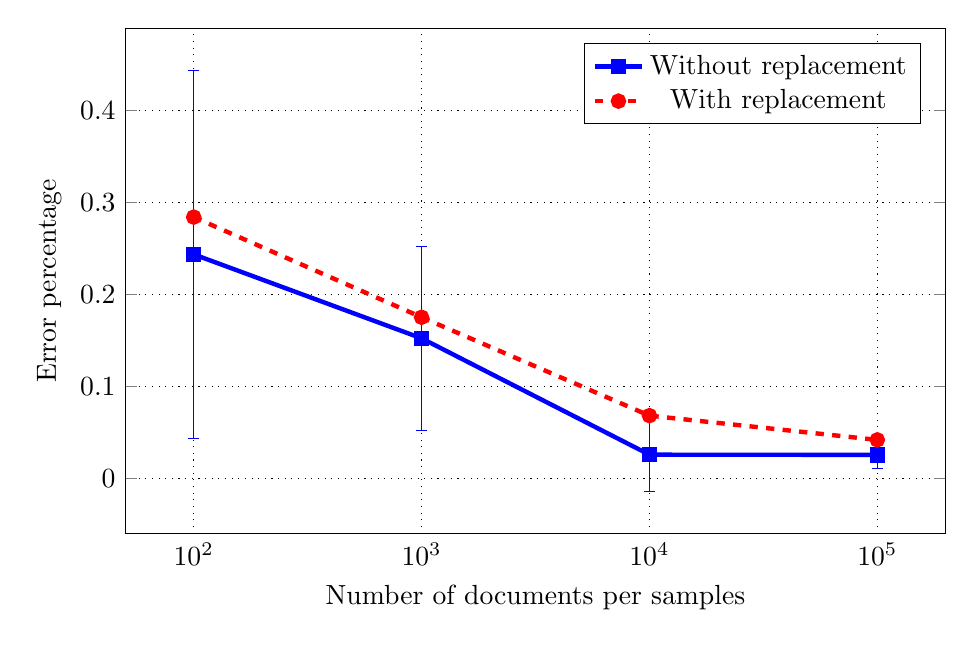
\begin{tikzpicture}
\begin{axis}[legend style={at={(0,0)},anchor=west,at={(axis description cs:1.05,0.45)}, every axis plot/.append style={ultra thick}},title={},
mark options={solid,scale=1},
xlabel={Number of documents per samples},
xmode = log,        % logarithmic x axis
ylabel={Error percentage},
%axis background/.style={fill,bottom color=gray!50,top color=white},
xtick style={draw=none},
grid=none,
height=8cm,width=12cm,
grid style={dotted,black},
legend pos=north east,
grid=major
]
\addplot[mark=square*,blue, error bars/.cd, y dir=both, y explicit] plot coordinates{
(100,0.243875) +=(0,0.2) -= (0,0.2)
(1000,0.152625) +=(0,0.1) -= (0,0.1)
(10000,0.0261373737) +=(0,0.04) -= (0,0.04)
(100000,0.026) +=(0,0.015) -= (0,0.015)
};
\addlegendentry{Without replacement}
\addplot[dashed,mark=*,red, error bars/.cd, y dir=both, y explicit] plot coordinates{ 
(100,0.284375)
(1000,0.175508425)
(10000,0.0686)
(100000,0.0422475)
};
\addlegendentry{With replacement}
\end{axis}
\end{tikzpicture}}
\caption{Error percentage with respect to sample sizes ($10^2$, $10^3$, $10^4$, $10^5$ documents per sample). Samples without replacement exhibit slightly more accurate results than samples with replacement.}
\label{errorPercentageFigure}
\end{figure}

%*************************************************
\subsection{Results and discussion}
\label{ResultAndDiscussionSubSection}
%*************************************************

\noindent \textbf{ Experimental setup.} We set up a cluster of $100$ AWS EC2 instances (t2.large) as homogeneous physical machines with $2$ vCPU, $8$ GB memory, and the Linux kernel version 4.4.0-59-generic has been utilized for experiments. For unmodified NoSQL server, MongoBD version 3.2.7 has been used as the NoSQL database server. The OPE and DHOM cryptosystems are implemented locally and other crypto modules are implemented from OpenSSL version 1.0.2g. The measured query latency time is considered as the interval between the time when the sever receives a query and the time it starts to forward the query result. For accurate measurement of the query latency, the query caching and pre-fetching disabled because, most of database servers keep all of the most recently used data in main memory, so the next matching queries will be served from memory accordingly. Furthermore, MongoDB supports variety of storage engines which are designed and optimized for various workloads. The storage engine is responsible for data storage both in memory and on disk. We chose \emph{WiredTiger} storage engine that is well-suited for the most of workloads.\\



\noindent \textbf{ AQP based sensitivity analysis.} The goal of sensitivity analysis here is to identify different document classes (i.e. Top Secret, Confidential, etc.), and their corresponding count and percentage. The result of the sensitivity analysis will be used to determine the number of disinformation documents to be added according to the level of document sensitivity. 

In the experiment, we used a database of ten million documents. Table \ref{tab:documentClass} shows the eight sensitivity levels and the number and percentage of documents in each sensitivity class.   

\begin{table*}[htp]
\caption{Document classification}
\label{tab:documentClass}
\centering
\begin{tabular}{lrl}
\toprule
\textbf{Class ($s_i$)} & \textbf{Cardinality($c_i$)} & \textbf{Percentage}\\
\midrule
Top Secret  & 782471  & 07.823\%  \\ 
Secret      & 1475118 & 14.751\% \\
Information & 3134844 & 31.348\% \\
Official    & 1475603 & 14.756\% \\
Unclassified& 783443  & 07.834\% \\
Clearance   & 783024  & 07.830\% \\
Confidential& 782698  & 07.826\% \\
Restricted  & 782799  & 07.828\% \\
\midrule
\textbf{Total}  & \textbf{10000000}  & \textbf{100.00\%} \\
\bottomrule
\end{tabular}
\end{table*}

We use aggregate query to compute the count and percentage of each class of documents in the collection. Let $\theta$ be an aggregate query required to compute over the dataset described in Table \ref{tab:documentClass}. For instance, consider query $\theta$ shown in Figure \ref{fig:aggregate}, which returns the count and percentage of each class of documents based on their security level.

%Figure 
\begin{figure}[H]
\begin{framed}
{\ttfamily \small{ 
\textbf{db[collection].aggregate}([\\
\{\textbf{"\$group":}\{"\_id":\{"clearance":"\$clearance"\},\\ \textbf{"count":}\{"\$sum":1\}\}\},\\
\{\textbf{"\$project":} \{  "count": 1, "percentage":\{
\textbf{"\$concat":}[\{\textbf{"\$substr":}[\\\{\textbf{"\$multiply":}[\{\textbf{"\$divide":}["\$count", \{"\$literal":Sample size \}]\},100]\}, 0,6]\},"", "\%"]\}\}\}\\]);
}
}
\end{framed}
\caption{Aggregate query $\theta$ for sensitivity analysis of collection. This query will be executed on the original database and $100$ sample databases.}
\label{fig:aggregate}
\end{figure}


The results show that the average speedup due to AQP is better than linear. A remarkable improvement in processing time and speedup is achieved and the price to pay for it is an acceptable level of inaccuracy. Both metrics are plotted against variant sample size in Figure \ref{fig:performance}. For the largest sample of $10^5$ documents, the average processing time is $93$ ms, whereas for the original database (including $10^7$ documents) the processing time of the same query is $14,000$ ms, a drastic improvement. The speedup of $150$ for this sample versus  the original database is remarkable. The approximated value for each class of documents are presented in Table \ref{tab:AproximatedDocumentClass}, which indicates $1300$ times speed up with the cost of less than 1\% error by using sample size of $10^4$. It is worthy to compare the result with the exact values of document classification listed in Table \ref{tab:documentClass}. As a result, AQP is a powerful method to substantially reduce query latency for very small cost of inaccuracy.  
 
\begin{figure}[H]
\begin{subfigure}{0.40\textwidth}
\centering
\resizebox{1.0\textwidth}{!}{\begin{tikzpicture}%[trim axis right, trim axis right]
\begin{axis}[
every axis plot post/.style={/pgf/number format/fixed},
ybar=5pt,
%enlarge y limits={upper,value=0.2},
height=6.5cm,width=12cm,
axis on top,
ymax=100,
bar width=15pt,
x=1.2cm,
symbolic x coords={$10^2$,$10^3$,$10^4$,$10^5$,$10^7$,$10^8$},
restrict y to domain*=0:110, % Cut values off at 110
visualization depends on=rawy\as\rawy, % Save the unclipped values
after end axis/.code={ % Draw line indicating break
\draw [ultra thick, white, decoration={snake, amplitude=1pt}, decorate] (rel axis cs:0,1.05) -- (rel axis cs:1,1.05);},
nodes near coords={%
\pgfmathprintnumber{\rawy}% Print unclipped values
},
axis lines*=left,
clip=false,
ylabel={Processing time(ms)},
xtick=data,
enlarge x limits=0.5,
xlabel={Number of documents per samples},
cycle list = {white,black!10,black!40,black!10,black!10}
]
\addplot+[fill,draw=black,text=black, postaction={pattern=crosshatch},draw=black] coordinates {({$10^2$},0.45) ({$10^3$},1.8) ({$10^4$},10.8) ({$10^5$},93) ({$10^7$},14000)};
\end{axis}
\end{tikzpicture}}
\label{fig:runTime}
\caption{}
\end{subfigure}
\qquad 
\begin{subfigure}{0.5\textwidth}
\resizebox{1.0\textwidth}{!}{\begin{tikzpicture}[trim axis right, trim axis right]
\begin{axis}[
legend pos=outer north east,
ybar,
%enlarge y limits={upper,value=0.2},
height=8cm,width=12cm,
ytick={1000,10000,20000,30000,40000,50000},
bar width=15pt,
ylabel={Speed up},
symbolic x coords={$10^2$,$10^3$,$10^4$,$10^5$,$10^7$,$10^8$},
xtick=data,
xtick style={draw=none},
nodes near coords,
nodes near coords align={vertical},
xmajorgrids=false,
xlabel={Number of documents per samples},
%axis background/.style={fill,bottom color=gray!50,top color=white},
cycle list = {white,black!10,black!40,black!10,black!10},
grid style={dotted,black},
axis lines*=left,
clip=false,
nodes near coords align={vertical},
yticklabel style={/pgf/number format/fixed},
]
\addplot+[fill,draw=black,text=black, postaction={pattern=north west lines},draw=black] coordinates {({$10^2$},31000) ({$10^3$},8000) ({$10^4$},1300) ({$10^5$},150)};
\end{axis}
\end{tikzpicture}}
\label{fig:speedup}
\caption{}
\end{subfigure}
\caption{The performance analysis of AQP: (a) processing time of aggregate query over the samples with different sizes; (b) significant speed up obtained by application of AQP for processing aggregate queries on samples for document classification. In this case $100$ random samples with $10^2, 10^3, 10^4$ and $10^5$ documents are examined.}
\label{fig:performance}
\end{figure}

\begin{table*}[h!]
\caption{Approximated values for each class of clearance level using sample size $10^4$.}
\label{tab:AproximatedDocumentClass}
\centering
\begin{tabular}{lrlr}
\toprule
\textbf{Class($s_j^\prime$)} & \textbf{Cardinality($c_j^\prime$)} & \textbf{Percentage} & \textbf{Deviation}\\
\midrule
Top Secret  & 785600  & 07.856\%   & -3129  \\ 
Secret      & 1462000 & 14.620\%   & 13118\\
Information & 3152200 & 31.522\%   & -17356\\
Official    & 1463700 & 14.637\%   & 11903 \\
Unclassified& 787200  & 07.872\%   & -3757 \\
Clearance   & 784800  & 07.848\%   & -1776 \\
Confidential& 783900  & 07.839\%   & -1202  \\
Restricted  & 780300  & 07.803\%   & -2499\\
\midrule
\textbf{Total}  & \textbf{9945260}  & \textbf{99.4526\%} & \textbf{54740}\\
\bottomrule
\end{tabular}
\end{table*}


\noindent {\bf Discussion.} In the previous section, an AQP-based sensitivity analysis was performed for eight hypothetical sensitivity classes and the relative error formulated according to Equation \ref{equ:RelativeError}. In our experiments, we considered eight sensitivity classes for AQP using $100$ uniform random samples (with variety of sampling rates from $0.001\%$  to $1\%$ ) form a database containing  $10^7$ documents. All of the samples have been selected to have the same size; so that, the processing time of the aggregate queries is within small range. AWS EC2 (t2.large) instances were used to process each sample. In general, the average speed up for a set of uniform random samples with $10^4$ documents is approximately $1300$x faster than the original database with $0.04\% \pm 0.02$ error percentage. Therefore, replacing the exact query with approximate query saves a remarkable amount of processing time, with a small cost of inaccuracy.

The AQP with uniform random sampling provides very reasonable results for classification aggregate query workload, with compromise between sample size and query latency. However, for queries with different workloads such as aggregate functions that involve multiple correlated databases, the uniform sampling cannot provide accurate responses and we designed a new technique for biased sampling solution for this problem. In the next section we highlight approximated answers for correlated databases.